\documentclass[t]{beamer}
\usetheme[deutsch]{KIT}
\setbeamercovered{transparent}
\setbeamertemplate{navigation symbols}{}

\KITfoot{Tutoriumsmaterial von Michael Vollmer}
\usepackage[utf8]{inputenc}
\usepackage{amsmath}
\usepackage{ifthen}
\usepackage{amssymb}
\usepackage{tikz}
\usepackage{ngerman}
\usepackage[normalem]{ulem}
\usepackage{stmaryrd}
\usetikzlibrary{automata}
\usenavigationsymbols
\usepackage{mathtools}
\usepackage{array}
\usepackage{colortbl}

\title{Theoretische Grundlagen der Informatik}
\subtitle{Tutorium}
\author{Michael Vollmer}

\institute[IKS]{Institut für Kryptographie und Sicherheit}

\TitleImage[height=\titleimageht]{images/tmaschine.png}

\newcommand{\N}{\ensuremath{\mathbb{N}}}
\newcommand{\M}{\ensuremath{\mathcal{M}}}
\newcommand{\classP}{\ensuremath{\mathcal{P}}}
\newcommand{\classNP}{\ensuremath{\mathcal{NP}}}
\newcommand{\co}{\ensuremath{\mathsf{co\text{-}}}}
\newcommand{\pot}{\ensuremath{\mathcal{P}}}
\newcommand{\abs}[1]{\ensuremath{\left\vert #1 \right\vert}}
\newcommand{\menge}[2]{\ensuremath{\left\lbrace #1 \,\middle\vert\, #2 \right\rbrace}}
\newcommand{\ducttape}[1]{\vspace{#1}}
\newcommand{\neglit}[1]{\overline{#1\vphantom{x^a}}}
\newcommand{\recipe}{\raisebox{-.3cm}{
\includegraphics[scale=.15]{images/chefs-cap.png}}\hspace{0.2cm}}
\newcommand{\opt}[1]{\ensuremath{\text{OPT}(#1)}}
\newcommand{\A}[1]{\ensuremath{\mathcal{A}(#1)}}
\renewcommand{\O}[1]{\ensuremath{\mathcal{O}(#1)}}
\newcommand{\msout}[1]{\text{\sout{\ensuremath{#1}}}}

\newcommand{\invincible}{\setbeamercovered{invisible}} %  "Yesss! I am invincible!!" (Boris Grishenko)
\newcommand{\vincible}{\setbeamercovered{transparent}}
\renewcommand{\solution}[1]{\invincible \pause #1 \vincible}
\newcommand{\micropause}{\\[8pt]}

% \@ifundefined{tikzset}{}{\tikzset{initial text=}} % Text "start" bei Startknoten unterdrücken
\tikzstyle{every node}=[thick]
\tikzstyle{every line}=[thick]

\newcommand{\tutnr}[1]{
  \subtitle{Tutorium #1}
	\begin{frame}
		\maketitle
	\end{frame}
}

\newcommand{\uebnr}[1]{
  \subtitle{Anmerkungen zum #1. Übungsblatt}
	\begin{frame}
		\maketitle
	\end{frame}
}

\begin{document}

\newcommand{\start}[3]
{
  \draw (#1*2,#2*2) node{$#3$};
  \draw (#1*2,#2*2) circle(0.4cm);
  \draw [->] (#1*2-0.9,#2) -- (#1*2-0.4,#2);
}
\newcommand{\final}[3]
{
  \draw (#1*2,#2*2) node{$#3$};
  \draw (#1*2,#2*2) circle(0.4cm);
  \draw (#1*2,#2*2) circle(0.32cm);
}
\newcommand{\startfinal}[3]
{
  \draw (#1*2,#2*2) node{$#3$};
  \draw (#1*2,#2*2) circle(0.4cm);
  \draw (#1*2,#2*2) circle(0.32cm);
  \draw [->] (#1*2-0.9,#2) -- (#1*2-0.4,#2);
}
\newcommand{\state}[3]
{
  \draw (#1*2,#2*2) node{$#3$};
  \draw (#1*2,#2*2) circle(0.4cm);
}
\newcommand{\tol}[4]
{
  \draw (#1+#3,#2*2) node[above]{$#4$};
  \draw [->] (#1*2-0.4,#2*2) -- (#3*2+0.4,#2*2);
}
\newcommand{\tor}[4]
{
  \draw (#1+#3,#2*2) node[above]{$#4$};
  \draw [->] (#1*2+0.4,#2*2) -- (#3*2-0.4,#2*2);
}
\newcommand{\tot}[4]
{
  \draw (#1*2,#2+#3) node[right]{$#4$};
  \draw [->] (#1*2,#2*2+0.4) -- (#1*2,#3*2-0.4);
}
\newcommand{\tob}[4]
{
  \draw (#1*2,#2+#3) node[right]{$#4$};
  \draw [->] (#1*2,#2*2-0.4) -- (#1*2,#3*2+0.4);
}
\newcommand{\totl}[5]
{
  \draw (#1+#3,#2+#4) node[above right]{$#5$};
  \draw [->] (#1*2-0.283,#2*2+0.283) -- (#3*2+0.283,#4*2-0.283);
}
\newcommand{\totr}[5]
{
  \draw (#1+#3,#2+#4) node[above left]{$#5$};
  \draw [->] (#1*2+0.283,#2*2+0.283) -- (#3*2-0.283,#4*2-0.283);
}
\newcommand{\tobl}[5]
{
  \draw (#1+#3,#2+#4) node[below right]{$#5$};
  \draw [->] (#1*2-0.283,#2*2-0.283) -- (#3*2+0.283,#4*2+0.283);
}
\newcommand{\tobr}[5]
{
  \draw (#1+#3,#2+#4) node[below left]{$#5$};
  \draw [->] (#1*2+0.283,#2*2-0.283) -- (#3*2-0.283,#4*2+0.283);
}
\newcommand{\rloopl}[3]
{
  \draw (#1*2-1,#2*2) node[left]{$#3$};
  \draw [->] (#1*2-0.35,#2*2-0.2) arc (-30:-320:0.32cm);
}
\newcommand{\rloopr}[3]
{
  \draw (#1*2+1,#2*2) node[right]{$#3$};
  \draw [->] (#1*2+0.35,#2*2+0.2) arc (150:-140:0.32cm);
}
\newcommand{\rloopt}[3]
{
  \draw (#1*2,#2*2+1) node[above]{$#3$};
  \draw [->] (#1*2-0.2,#2*2+0.35) arc (240:-50:0.32cm);
}
\newcommand{\rloopb}[3]
{
  \draw (#1*2,#2*2-1) node[below]{$#3$};
  \draw [->] (#1*2+0.2,#2*2-0.35) arc (60:-230:0.32cm);
}
\newcommand{\lloopl}[3]
{
  \draw (#1*2-1,#2*2) node[left]{$#3$};
  \draw [->] (#1*2-0.35,#2*2+0.2) arc (30:320:0.32cm);
}
\newcommand{\lloopr}[3]
{
  \draw (#1*2+1,#2*2) node[right]{$#3$};
  \draw [->] (#1*2+0.35,#2*2-0.2) arc (-150:140:0.32cm);
}
\newcommand{\lloopt}[3]
{
  \draw (#1*2,#2*2+1) node[above]{$#3$};
  \draw [->] (#1*2+0.2,#2*2+0.35) arc (-60:230:0.32cm);
}
\newcommand{\lloopb}[3]
{
  \draw (#1*2,#2*2-1) node[below]{$#3$};
  \draw [->] (#1*2-0.2,#2*2-0.35) arc (-240:50:0.32cm);
}
\tutnr{5}

\section{Übungsblatt 1}
\subsection{Übungsblatt 1}

\begin{frame}
\frametitle{Best of Übungsblatt 2}
\begin{itemize}
	\item Abgaben: 16 von 21 (76,2\%)
	\item Mindestens 50\% Punkte: 14 von 16 (87.5\%)
	\item Durchschnittliche erreichte Punktzahl: 9.65
	\begin{itemize}
		\item (nach Aufrunden auf halbe Punkte)
	\end{itemize}
\end{itemize}~\\~\\~\\
Aufgabenverteilung
\begin{enumerate}[{A}ufg{a}be 1:]
	\item Gesamt: 51.75P (durchscnittlich 3.23)
	\item Gesamt: 53P (durchschnittlich 3.31)
	\item Gesamt: 37.25P (durchschnittlich 2.32)
	\item Gesamt: 8.25 (durchschnittlich 0.52)
\end{enumerate}
\end{frame}

\section{Turingmaschine}
\subsection{Allgemeine Turingmaschine}
\subsection{Turingmaschine}
\begin{frame}
	\frametitle{Turingmaschine}
	Die Turingmaschine besteht aus einem beidseitig \emph{unendlichen} Eingabe- und Rechenband
	mit einem frei beweglichen Lese-/Schreibkopf, der von einer \emph{endlichen} Kontrolle gesteuert wird. 
	\begin{center}
		\vspace{1cm}
		\hspace{-12mm}
		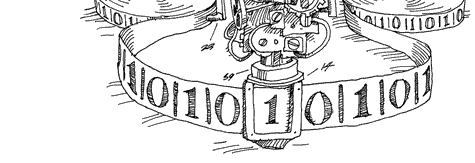
\includegraphics[scale=0.5]{images/tmaschine.png}
	\end{center}
\end{frame}
\begin{frame}
\frametitle{Turingmaschine}
\begin{block}{Definiton}
Eine Turingmaschine wird definiert als ein 7-Tupel bestehend aus:
 \begin{itemize}
 \item $Q$, einer endlichen Zustandsmenge
 \item $\Sigma$, einem endlichen Eingabealphabet
 \item $\Gamma$, einem endlichen Bandalphabet mit $\Sigma \cup\{\sqcup\} \subseteq \Gamma$, wobei $\sqcup \notin \Sigma$
 \item $\delta$, einer Übergangsfunktion $\delta: Q\times\Gamma \rightarrow Q\times\Gamma\times\{L, R, N\}$
 \item $s \in Q$, einem Startzustand
 \item $q_{accept}$, einem akzeptierenden Zustand
 \item $q_{reject}$, einem ablehnenden Zustand
 \end{itemize}
\end{block}
\begin{block}{Bemerkung}
 In den Zuständen $q_{accept}$ und $q_{reject}$ hält die Turingmaschine unabhängig davon, was vom Band eingelesen wird. Zudem führen alle impliziten Übergänge in den Zustand $q_{reject}$.
\end{block}
\end{frame}

\frame{
	\frametitle{Graph einer Turingmaschine}
	\begin{center}
	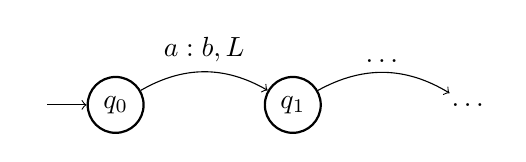
\begin{tikzpicture}[node distance=2.25cm,auto]
	\node(q0)[draw,circle,thick]{$q_0$};
	\node (s) [node distance=1cm,left of =q0]{};
	\node(q1)[draw,circle,thick,right of=q0]{$q_1$};
	\node(qx)[right of=q1]{\dots};

	\path[->]       (s) edge (q0)
	                (q0) edge[bend left] node{$a:b,L$} (q1)
			                (q1) edge[bend left] node{\dots} (qx);
					\end{tikzpicture}
					\end{center}

					Dabei steht die Kantenbeschriftung "`$a:b,L$"' für den Übergang $\delta(q_0,a) =
					(q_1,b,L)$.

					\vspace{2mm}
					Falls es für einen gegebenen Zustand und ein gegebenes
					Symbol keinen Zustandsübergang gibt, bricht die Maschine die Berechnung ab, bzw. geht in Zustand $q_{reject}$ über.
}

\begin{frame}
\frametitle{Konfigurationen}
Sei $\mathcal{M} =(Q,\Sigma, \Gamma,\delta,s,q_{accept},q_{reject})$ eine Turingmaschine.

Angabe des aktuellen Berechnungszustandes: \emph{Konfiguration}

$$w(q)av$$ 

wobei $w,v \in \Gamma^*, a \in \Gamma$ und $q\in Q$. \\

Dies bedeutet:

\begin{itemize}
	\item $\mathcal{M}$ befindet sich im Zustand $q$.
	\item Der Lesekopf steht auf dem Zeichen $a$.
	\item Links vom Lesekopf steht das Wort $w$ und rechts davon das Wort $v$ auf dem Rechenband.
\end{itemize}
\end{frame}

\subsection{Aufgaben deterministische Turingmaschine}
\begin{frame}
\frametitle{Aufgabe B4 2.2}
Gegeben sei folgende deterministische Turingmaschine $\mathcal{TM} =
(\mathcal{Q},\Sigma,\Gamma,\delta,q_0,\#,\mathcal{F})$, wobei $\Sigma = \{a,b\}$,
$\Gamma = \Sigma \cup \{B,\#\}$, den Zust"anden $\mathcal{Q} = \{q_0,\dots,q_7\}$,
dem Startzustand $q_0$, den Finalzust"anden $\mathcal{F} = \{q_7\}$ und dem
Bandzeichen $\#$. Der Zustands"ubergangsgraph ist gegeben durch:
\begin{center}
\resizebox{10cm}{!} {
\begin{tikzpicture}[line width=1pt]
\start{0}{0}{q_0}
\tob{0}{0}{-2}{(a,\#,R)}
\tor{0}{0}{3.5}{(B,\#,R)}
\draw (2,-2) node[above right]{$(\#,\#,N)$};
\draw [->] (0.283,-0.283) -- (3.717,-3.717);
\state{0}{-2}{q_1}
\rloopb{0}{-2}{(a,a,R),(B,B,R)}
\tol{0}{-2}{-2}{(b,B,L)}
\state{-2}{-2}{q_2}
\rloopb{-2}{-2}{(a,a,L),(B,B,L)}
\totr{-2}{-2}{0}{0}{(\#,\#,R)}
\state{3.5}{0}{q_3}
\rloopt{3.5}{0}{(a,a,R),(B,B,R)}
\tor{3.5}{0}{5}{(\#,\#,L)}
\state{5}{0}{q_4}
\tob{5}{0}{-2}{(a,\#,L)}
\state{5}{-2}{q_5}
\rloopb{5}{-2}{(a,a,L),(B,B,L)}
\tol{5}{-2}{3.5}{(\#,\#,R)}
\state{3.5}{-2}{q_6}
\tot{3.5}{-2}{0}{(B,\#,R)}
\tol{3.5}{-2}{2}{(\#,\#,N)}
\final{2}{-2}{q_7}
\end{tikzpicture}
}
\end{center}
Finden Sie die Sprache, die von der Turingmaschine $\mathcal{TM}$ akzeptiert wird!
\end{frame}
\begin{frame}
	\frametitle{Aufgabe B5 3}
	Geben Sie f"ur die nachfolgenden Sprachen "uber dem Alphabet $\Sigma = \{0,1\}$
	jeweils eine Turingmaschine an, die die entsprechende Sprache akzeptiert!
	\begin{enumerate}
		\item $\mathcal{L} = \{ \omega \in \{0,1\}^* \; | \; \omega \;
		\mbox{enth"alt das Zeichen $0$ gleich oft wie das Zeichen $1$} \}$
		\item $\mathcal{L}' = \{ \omega \in \{0,1\}^* \; | \; \omega \;
		\mbox{enth"alt das Zeichen $0$ doppelt so oft wie das Zeichen $1$} \}$
		\item $\mathcal{L}'' = \{ \omega \in \{0,1\}^* \; | \; \omega \;
		\mbox{enth"alt das Zeichen $0$ nicht doppelt so oft wie das Zeichen $1$} \}$
	\end{enumerate}
\end{frame}

\subsection{Nichtdeterministische Turingmaschine}
\begin{frame}
	\frametitle{Nichtdeterministische Turingmaschine}
	Was ist das?
	\begin{itemize}
		\item Wie eine normale Turingmaschine...
		\item ... nur nicht-deterministisch.
	\end{itemize}
	Soll heißen:
	\begin{itemize}
		\item Mehrere Übergänge für das selbe gelesene Zeichen in einem Zustand
		\item akzeptiert wird, wenn es eine Berechnungsfolge gibt die in $q_{accept}$ endet
	\end{itemize}
	~\\~\\~\\
	Kurz gesagt:~\\
	Analog zu Automaten, nur ohne $\epsilon$-Übergänge.
\end{frame}

\subsection{Aufgaben nichtdeterministische Turingmaschine}
\begin{frame}
\frametitle{Aufgabe B4 2.1}
Geben Sie eine nichtdeterministische Turingmaschine $\mathcal{TM} =
(\mathcal{Q},\Sigma,\Gamma,\delta,q_0,\square,\mathcal{F})$ an, welche die Sprache
$\mathcal{L} = \{ww \; | \; w \in \{a,b\}^*\}$ erkennt! Es gen"ugt dabei, den
Zustands"ubergangsgraphen zu zeichnen und das verwendete Bandalphabet anzugeben.
\end{frame}

\subsection{Linear beschränkte Turingmaschine}
\begin{frame}
	\frametitle{Linear beschränkte Turingmaschine}
	Eine linear beschränkte Turingmaschine (auch \emph{LBA} = Linear Bounded Automaton) darf den Bereich des Bandes auf dem die Eingabe steht nicht verlassen bzw. maximal das erste Blank-Symbol rechts der Eingabe verwenden.\\
	\vspace{2mm}
	Variation:
	\begin{itemize}
		\item Die linear beschränkte Turingmaschine darf noch genau ein weiteres Zeichen rechts von dem Eingabewort zu verwenden. 
	\end{itemize}
	\vspace{2mm}
	Die von der nichtdeterministischen linear beschränkten Turingmaschine akzeptierten Sprachen sind genau die kontextsensitiven Sprachen. (CH-1)
\end{frame}

\subsection{Aufgabe linear beschränkte Turingmaschine}
\begin{frame}
\frametitle{Aufgabe B4 1}
\begin{enumerate}
\item Geben Sie f"ur die Sprache $\mathcal{L}' = \{a^{2^n} \; | \; n \in
\mathbb{N}\}$ eine linear beschr"ankte Turing-Maschine an und zeichnen\\
Sie diese Turing-Maschine auch als Graphen!
\item Pr"ufen Sie, ob Ihre Turing-Maschine $aaaa$ als Eingabe akzeptiert!
Pr"ufen Sie auch nach, ob $aaa$ \underline{nicht}\\
akzeptiert wird!
\end{enumerate}
\end{frame}

\section{Chomsky-Hierarchie}
\subsection{Chomsky-Hierarchie}
\begin{frame}
	\frametitle{Grammatiken}
Eine kontextsensitive Grammatik $G = ( T, V, S, P)$ (Chomsky Typ 1)
\begin{itemize}
	\item $T$ = Menge der Terminale (a.k.a. Alphabet der Sprache)
	\item $V$ = Menge der Nichtterminale (zu T disjunkt)
	\item $S \in V$ = Startsymbol
	\item $P$ = Menge der Produktionen mit Form $v \rightarrow w$
	\begin{itemize}
		\item $v \in V^{+}$
		\item $w \in ((V \setminus \{S\}) \bigcup T)^{+}$
		\item $|v| \leq |w|$ oder $S \rightarrow \epsilon$
	\end{itemize}
\end{itemize}~\\~\\




Eine Grammatik $G = ( T, V, S, P)$ (Chomsky Typ 0)
\begin{itemize}
	\item $T$ = Menge der Terminale (a.k.a. Alphabet der Sprache)
	\item $V$ = Menge der Nichtterminale (zu T disjunkt)
	\item $S \in V$ = Startsymbol
	\item $P$ = Menge der Produktionen mit Form $v \rightarrow w$
	\begin{itemize}
		\item $v,w \in (V \bigcup T)^{*}$
	\end{itemize}
\end{itemize}
\end{frame}

\begin{frame}
	\frametitle{Chomsky-Hierarchie}
	\begin{itemize}
		\item \textbf{Chomsky Typ 3}
		\begin{itemize}
			\item Reguläre Sprachen (z.B. rechtslineare Sprachen)
			\item Reguläre Ausdrücke
			\item Endliche Automaten
		\end{itemize}
		\item \textbf{Chomsky Typ 2}
		\begin{itemize}
			\item $Ch3 \subseteq Ch2$
			\item Kontextfreie Sprachen
			\item Nichtdeterministische Kellerautomaten
			\item Programmiersprachen sind in der Regel $Ch2$
		\end{itemize}
		\item \textbf{Chomsky Typ 1}
		\begin{itemize}
			\item $Ch2 \subseteq Ch1$
			\item Kontextsensitiven Sprachen
			\item Nichtdeterministische, linear platzbeschränkte Turingmaschine
		\end{itemize}
		\item \textbf{Chomsky Typ 0}
		\begin{itemize}
			\item $Ch1 \subseteq Ch0$
			\item Grammatiken mit beliebiger Produktionsmenge
			\item Semi-entscheidbare Sprachen (durch Turingmaschine)
			\item rekursiv aufzählbare Sprachen
		\end{itemize}
	\end{itemize}
\end{frame}

\section{Schluss}
\subsection{Schluss}
\begin{frame}
\frametitle{Bis zum nächsten Mal!}
\begin{center}
  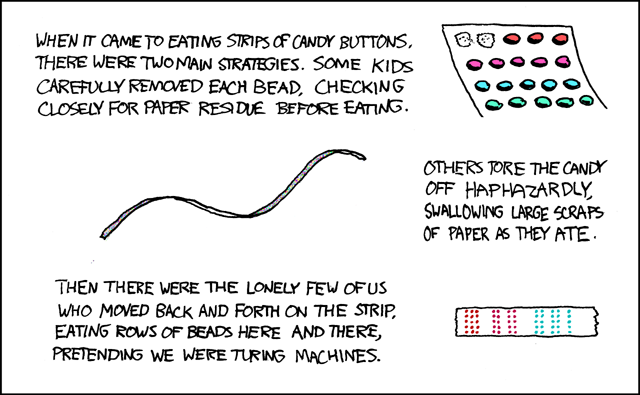
\includegraphics[width=1 \textheight]{images/xkcd_205.png}
\end{center}
\end{frame}

\frame{
  \frametitle{Lizenzen}
  \center
  
\includegraphics[width=2em]{images/by}
  
\includegraphics[width=2em]{images/cc}
  
\includegraphics[width=2em]{images/sa}
  \\
  {\tiny

Dieses Werk ist unter einem ``Creative Commons Namensnennung-Weitergabe unter gleichen Bedingungen 3.0 Deutschland``-Lizenzvertrag lizenziert. Um eine Kopie der Lizenz zu erhalten, gehen Sie bitte zu \href{http://creativecommons.org/licenses/by-sa/3.0/de/}{http://creativecommons.org/licenses/by-sa/3.0/de/} oder schreiben Sie an Creative Commons, 171 Second Street, Suite 300, San Francisco, California 94105, USA.\\
  \vspace{1cm}
  Davon ausgenommen sind das Titelbild, welches aus der März-April 2002 Ausgabe von American Scientist erschienen ist und ohne Erlaubnis verwendet wird, sowie das KIT Beamer Theme. Hierfür gelten die Bestimmungen der jeweiligen Urheber.
  \vspace{1cm}
  \\ 
  }
  %Habe hier die Reihenfolge etwas umgestellt, weil die Formatierung bei mir komisch aussah. 
  %Wenn es bei dir anders ist, kannst du es auch wieder zurückändern, dann haben wir unterschiedliche Kompilieroptionen
}

\end{document}